\documentclass[tikz,border=7pt]{standalone}
\usepackage{amsmath,amssymb}
\usetikzlibrary{arrows.meta,positioning}
\tikzset{vertex/.style={circle,draw,fill=cyan!12,minimum size=7mm,inner sep=1pt},box/.style={draw,rounded corners,fill=cyan!8,align=center,minimum height=12mm,minimum width=27mm}}
\begin{document}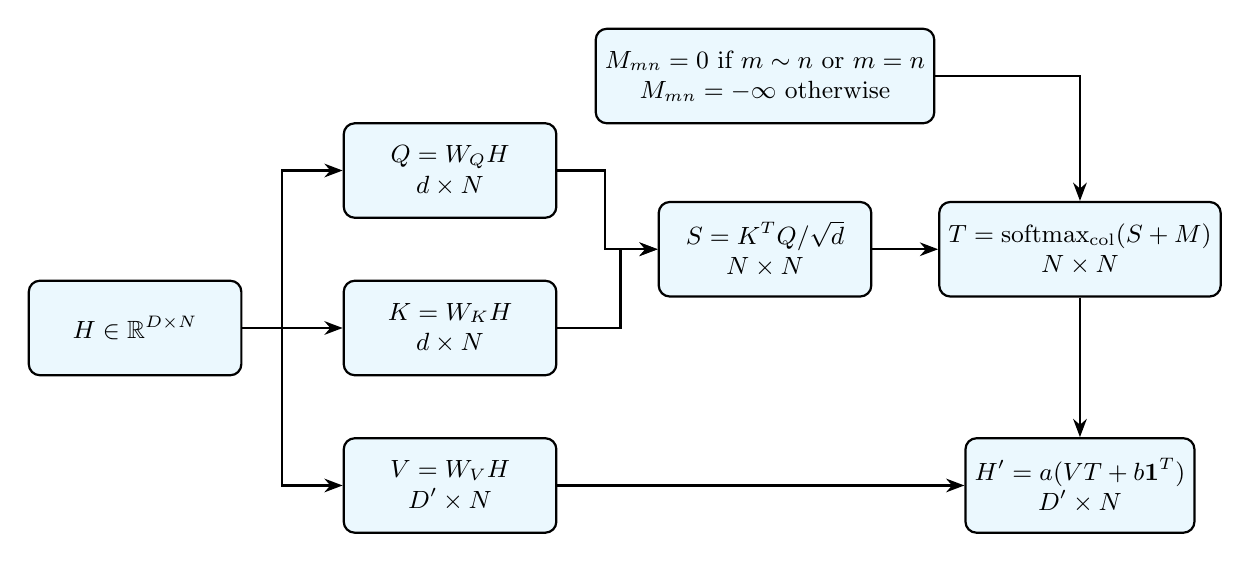
\begin{tikzpicture}[line width=0.8pt,font=\small]

\node[box] (h) at (0,0) {$H\in\mathbb R^{D\times N}$};
\node[box] (q) at (4,2) {$Q=W_QH$\\$d\times N$};
\node[box] (k) at (4,0) {$K=W_KH$\\$d\times N$};
\node[box] (v) at (4,-2) {$V=W_VH$\\$D'\times N$};
\node[box] (s) at (8,1) {$S=K^TQ/\sqrt d$\\$N\times N$};
\node[box] (mask) at (8,3.2) {$M_{mn}=0\text{ if }m\sim n\text{ or }m=n$\\$M_{mn}=-\infty\text{ otherwise}$};
\node[box] (att) at (12,1) {$T=\operatorname{softmax}_{\rm col}(S+M)$\\$N\times N$};
\node[box] (out) at (12,-2) {$H'=a(VT+b\mathbf1^T)$\\$D'\times N$};
\draw[-{Stealth}] (h.east) -- ++(0.5,0) |- (q.west);
\draw[-{Stealth}] (h.east) -- (k.west);
\draw[-{Stealth}] (h.east) -- ++(0.5,0) |- (v.west);
\draw[-{Stealth}] (q.east) -- ++(0.6,0) |- (s.west);
\draw[-{Stealth}] (k.east) -- ++(0.8,0) |- (s.west);
\draw[-{Stealth}] (s.east) -- (att.west);
\draw[-{Stealth}] (mask.east) -| (att.north);
\draw[-{Stealth}] (att.south) -- (out.north);
\draw[-{Stealth}] (v.east) -- (out.west);

\end{tikzpicture}\end{document}
